\documentclass[a4paper,landscape,8pt]{extarticle}

\usepackage[a4paper,margin=0.7cm]{geometry}

\usepackage{fancyhdr}
\pagestyle{fancy}
\fancyfoot[R]{\vspace{-35pt}\Huge\thepage}

\usepackage{multicol}
\setlength\columnsep{20pt}
\setlength{\columnseprule}{0.1pt} 

\setlength\parindent{0pt}

\usepackage[ngerman]{babel} % Silbentrennung
\usepackage[utf8]{inputenc} % Umlaute
\usepackage{microtype}

\usepackage{hyperref}

\usepackage{float}
\usepackage{graphicx}

\usepackage{comment}
\usepackage{amsmath}
\usepackage{amssymb}

\usepackage{cancel}

\usepackage{color}
\usepackage{xcolor}

\usepackage{color}

\usepackage{booktabs}

\newenvironment{rcases}
  {\left.\begin{aligned}}
  {\end{aligned}\right\rbrace}
  
\usepackage{enumitem}
\setlist{noitemsep,topsep=3pt,parsep=3pt,partopsep=3pt,leftmargin=18pt}
\renewcommand\labelitemi{{\boldmath$\cdot$}}
\newcommand{\listarrow}{
\smash{\scalebox{1.5}[1.75]{\rotatebox[origin=c]{180}{$\Lsh$}}}
}

\usepackage{xifthen}
\newcommand{\emptyarg}[1][]{\ifthenelse{\isempty{#1}}{}{\ #1}}

% % % % %
% Structural
% % % % %

\newcommand{\Def}[1][]{\colorbox{defcolor}{\color{titlecolor}{\textbf{D\emptyarg[#1]}}}\kern+0.3ex}

\newcommand{\Theorem}[1][]{\colorbox{satzcolor}{\color{titlecolor}{\textbf{T\emptyarg[#1]}}}\kern+0.3ex}

\newcommand{\Lemma}[1][]{\colorbox{lemcolor}{\color{titlecolor}{\textbf{L\emptyarg[#1]}}}\kern+0.3ex}

\newcommand{\Korollar}[1][]{\colorbox{lemcolor}{\color{titlecolor}{\textbf{K\emptyarg[#1]}}}\kern+0.3ex}

\newcommand{\Trick}[1][]{\colorbox{trkcolor}{\color{titlecolor}{\textbf{Trick:\emptyarg[#1]}}}\kern+0.3ex}

\newcommand{\Procedure}[1][]{\colorbox{trkcolor}{\color{titlecolor}{\textbf{Procedure:\emptyarg[#1]}}}\kern+0.3ex}

\newcommand{\Bsp}[1][]{\colorbox{bspcolor}{\color{titlecolor}{\textbf{B\emptyarg[#1]}}}\kern+0.3ex}

% % % % %
% In Text
% % % % %

\newcommand{\Bem}{\textbf{Bem: }}
\newcommand{\Beweis}{\textbf{Beweis: }}
\newcommand{\Achtung}{\textbf{Achtung: }}
\newcommand{\Wichtig}{\textbf{Wichtig: }}

% % % % %
% Colors
% % % % %

\definecolor{defcolor}{rgb}{0.5, 1, 0.5}
\definecolor{satzcolor}{rgb}{0.5, 0.95, 1}
\definecolor{lemcolor}{rgb}{1, 0.75, 0.75}
%\definecolor{trkcolor}{rgb}{1, 0.7, 0}
\definecolor{trkcolor}{rgb}{0.7, 0.95, 1}
\definecolor{bspcolor}{rgb}{1, 0.95, 0.43}
\definecolor{titlecolor}{rgb}{0,0,0}

% % % % %
% Math
% % % % %

\DeclareMathOperator{\arcsinh}{arcsinh}
\DeclareMathOperator{\arccosh}{arccosh}
\DeclareMathOperator{\arctanh}{arctanh}
\DeclareMathOperator{\arc}{arc}

\renewcommand\div{\operatorname{div}}
\DeclareMathOperator{\rot}{rot}
\newcommand{\laplace}{\Delta}

\DeclareMathOperator{\cis}{cis}

\DeclareMathOperator{\grad}{grad}
\DeclareMathOperator{\Hess}{Hess}

\newcommand{\N}{\mathbb{N}}
\newcommand{\Z}{\mathbb{Z}}
\newcommand{\Q}{\mathbb{Q}}
\newcommand{\R}{\mathbb{R}}
\newcommand{\C}{\mathbb{C}}

\renewcommand\Re{\operatorname{Re}}
\renewcommand\Im{\operatorname{Im}}

\newcommand{\abs}[1]{\left\lvert #1 \right\rvert}
\newcommand{\norm}[1]{\left\lVert #1 \right\rVert}
\newcommand{\scprod}[1]{\left\langle #1 \right\rangle}
\newcommand{\ceil}[1]{\left\lceil #1 \right\rceil}
\newcommand{\floor}[1]{\left\lfloor #1 \right\rfloor}

\newcommand{\diag}{\operatorname{diag}}

\newcommand{\hl}[1]{\colorbox{black!7}{$#1$}}

\newcommand{\notimplies}{\;\not\!\!\!\implies}

% % % % %
% Layout
% % % % %

\newcommand{\setsep}{\ \vert \ }

\newcommand{\todo}{\textcolor{red}{TODO }}

\newcommand{\sep}{\vspace{5pt}\noindent\hrule\vspace{5pt}}


\newcommand{\veryshortarrow}[1][3pt]{\mathrel{%
   \hbox{\rule[\dimexpr\fontdimen22\textfont2-.2pt\relax]{#1}{.4pt}}%
   \mkern-4mu\hbox{\usefont{U}{lasy}{m}{n}\symbol{41}}}}

% TODO remove command
\renewcommand*{\newpage}{ \ }

%\renewcommand*{\part}{\ }


% package to define custom environments
\usepackage{environ}

% boolean variable to show contents
\newif\ifshowwarmup
%\showwarmuptrue % set it to true
\showwarmupfalse % set it to false

% definition of custom environment
\NewEnviron{warmup}{\ifshowwarmup \BODY \fi}

% shorthand for custom environment
%\def\WU#1\UW{\begin{warmup}#1\end{warmup}}

% Ultra shortening of Document
%
% http://www.terminally-incoherent.com/blog/
%2007/09/19/latex-squeezing-the-vertical-white-space/
%\setlength{\parskip}{0pt}
%\setlength{\parsep}{0pt}
%\setlength{\headsep}{0pt}
\setlength{\topskip}{0pt}
%\setlength{\topmargin}{0pt}
%\setlength{\topsep}{0pt}
%\setlength{\partopsep}{0pt}
%\linespread{0.7}
\usepackage[compact]{titlesec}
\titlespacing{\section}{0pt}{*0}{*0}
\titlespacing{\subsection}{0pt}{*0}{*0}
\titlespacing{\subsubsection}{0pt}{*0}{*0}
%\usepackage{savetrees} %(alternative)

\pagenumbering{gobble}

% Use custom numbering
%\setcounter{secnumdepth}{0}

\usepackage{centernot}



\begin{document}

\setlength{\belowdisplayskip}{4pt} \setlength{\belowdisplayshortskip}{4pt}
\setlength{\abovedisplayskip}{4pt} \setlength{\abovedisplayshortskip}{4pt}

% allow page break in align* environment
\allowdisplaybreaks

\begin{multicols*}{4}
\raggedcolumns

\graphicspath{ {./img/} }

\sep
\section{Grundlagen}
\Satz[1.1.2]  $\R$ ist ein kommutativer, angeordneter Körper, der ordnungsvollständig ist
\sep

\subsection{Infimum und Supremum}
\Def[1.1.12]  Sei $A \subset \R$ eine Teilmenge.
\begin{enumerate}
\item[1)]  $c \in \R$ ist \textbf{obere Schranke} if  $\forall a \in A: a \leqslant c$
\item[2)]  $c \in \R$ ist \textbf{untere Schranke} if $\forall a \in A: c \leqslant a$
\item[3)] $m \in \R$ heisst ein \textbf{Maximum} von A if $m \in A$ und $m$ eine obere Schranke von A ist.
\item[4)] $m \in \R$ heisst ein \textbf{Minimum} von A if $m \in A$ und $m$ eine untere Schranke von A ist.  \\
\end{enumerate}

\Satz[1.1.15]. Sei $A \subset \R, A \neq \varnothing$ und beschränkt
\begin{enumerate}
\item[1)]  Kleinste obere Schranke: $\sup A$ (\textbf{Supremum})
\item[2)]  Grösste untere Schranke: $\inf A $ (\textbf{Infimum})  \\
\end{enumerate}

Eigenschaften von Supremum und Infimum
\begin{enumerate}
\item[•]  $\sup (A \cup B) = \text{max} (\sup A, \sup B)$
\item[•]  $\sup (A + B) = \sup A + \sup B$
\item[•]  $\inf (A \cup B) = \text{min} (\inf A, \inf B)$
\item[•]  $\inf (A + B) = \inf A + \inf B$
\end{enumerate}
\sep
\section{Folgen und Reihen}

\Def[2.1.1] Eine \textbf{Folge} $a_n$ in $\R$ ist eine Abbildung
\[
a: \N\longrightarrow \R
\] 
\sep
\subsection{Konvergenz von Folgen}

\Def[2.1.4] Eine Folge $a_n$ heisst \textbf{konvergent}, falls es $a \in \R$ gibt, so dass $\forall \epsilon > 0$ die Menge
$
\left\{n \in \N: a_{n} \notin\right] a-\varepsilon, a+\varepsilon[\}
$ endlich ist.
\Lemma[2.1.3] Dieses $a$ ist \textbf{eindeutig}. \\

\Lemma[2.1.5] Jede konvergente Folge ist \textbf{beschränkt}. \\
\Achtung $a_{n}$ beschränkt $\centernot\implies a_{n}$ konvergent! \\

\Lemma[2.1.6] Eine Folge $a_n$ \textbf{konvergiert} gegen ${a = \lim\limits_{n \rightarrow \infty} a_{n}}$, falls $ \forall \epsilon > 0 \ \exists N \geq 0$ so dass $\ \forall n\geq N$
\[
 \abs{a_n-a} < \epsilon.
\]

\Satz[2.1.8] Seien $a_n$ und $b_n$ konvergente Folgen mit $a = \lim\limits_{n \rightarrow \infty} a_{n}$ und  $b = \lim\limits_{n \rightarrow \infty} b_{n}$
\begin{enumerate}
\item[1)] Dann ist $\lim\limits_{n \rightarrow \infty} (a_{n} + b_{n}) = a + b$
\item[2)] Dann ist $\lim\limits_{n \rightarrow \infty} (a_{n} \cdot b_{n}) = a \cdot b$
\item[3)] Dann ist $\lim\limits_{n \rightarrow \infty} (\frac{a_{n}}{b_{n}}) = \frac{a}{b}$ $(b_{n} \neq 0 \ \forall n \geq 0)$
\item[4)] $\exists K \geq 0 \ \forall n \geq K \ a_{n} \leq b_{n} \implies a \leq b$

\end{enumerate}

\Satz[Sandwich Satz] Sei $\lim\limits_{n \rightarrow \infty} a_{n} = \lim\limits_{n \rightarrow \infty} b_{n} = \alpha$ 
\[
a_{n} \leq c_{n} \leq b_{n} \ \forall n \geq K \implies \lim\limits_{n \rightarrow \infty} c_{n} = \alpha
\]

Die Folge $a_{n}$ ist divergent, falls sie nicht konvergiert.
\sep

\subsection{Weierstrass und Anwendungen}

\Def[2.2.1] Falls  $a_{n}$ ist
\begin{enumerate}
\item[1)] \textbf{monoton wachsend}  falls ${a_{n} \leq a_{n + 1} \ \forall n \geq 0}$
\item[2)] \textbf{monoton fallend} falls ${a_{n} \geq a_{n + 1} \ \forall n \geq 0}$ \\
\end{enumerate}


\Satz[2.2.2 (Weierstrass)] Genau dann, wenn $a_{n}$ 
\begin{enumerate}
\item[1)] \textit{monoton wachsend} und \textit{nach oben beschränkt} ist, dann \textbf{konvergiert} $a_{n}$ mit Grenzwert
\[ 
\lim\limits_{n \rightarrow \infty} a_{n} = \text{sup}\{a_{n} \: n \geq 0\}
\]
\item[2)] \textit{monoton fallend} und \textit{nach unten beschränkt} ist, dann \textbf{konvergiert} $a_{n}$ mit Grenzwert
\[ 
\lim\limits_{n \rightarrow \infty} a_{n} = \text{inf}\{a_{n} \: n \geq 0\}
\]
\end{enumerate}
\Bsp[2.2.3] $\lim\limits_{n \rightarrow \infty} n^{a}q^{n} = 0, \ 0 \leq q < 1, \ a \in \Z$ \\
\Bsp[2.2.5] $\lim\limits_{n \rightarrow \infty} \sqrt[n]{n} = 1$ \\
\Bsp[2.2.6] $\lim\limits_{n \rightarrow \infty} (1 + \frac{1}{n})^n = e$ \\
\Lemma[2.2.7 (Bernoulli Ungleichung)]
\[
(1 + x)^{n+1} \geq 1 + n \cdot x \ \ \forall n \in \N, x > -1
\] 

\sep

\subsection{Limes superior und inferior}

\Def[2.3.0]
\[
\liminf\limits_{n \rightarrow \infty} a_{n} = \lim\limits_{n \rightarrow \infty} b_{n}, \ \ (b_{n} = \text{inf} \{a_{k} : k \geq n \})
\]
\[
\limsup\limits_{n \rightarrow \infty} a_{n} = \lim\limits_{n \rightarrow \infty} c_{n}, \ \ (c_{n} = \text{sup} \{a_{k} : k \geq n \})
\]


\Lemma[2.4.1] Die Folge $a_{n}$ konvergiert genau dann, falls
\begin{enumerate}
\item[1.] $a_{n}$ beschränkt ist
\item[2.] $\limsup\limits_{n \rightarrow \infty} a_{n} = \liminf\limits_{n \rightarrow \infty} a_{n}$
\end{enumerate}

\sep 

\subsection{Cauchy Kriterium}

\Satz[2.4.2 (Cauchy Kriterium)] Die Folge $a_{n}$ ist genau dann konvergent und heisst Cauchy-Folge
\[
\forall \epsilon > 0 \ \exists N \geq 0 \text{ so dass } \abs{a_{n} - a_{m}}  < \epsilon \ \ \forall n, m \geq N
\]

\sep

\subsection{Bolzano-Weierstrass}

\Def[2.5.1] Ein abgeschlossenes Intervall $I \subset \R$ 
\begin{enumerate}
\item[1)] $\left[ a, b \right]$, $a \leq b, a, b \in \R$
\item[2)] $\left[ a, +\infty \right[$, $a \in \R$
\item[3)] $\left] -\infty, a \right]$, $a \in \R$
\item[4)] $\left] -\infty, +\infty \right] = \R$
\end{enumerate}

Die Länge eines $\mathcal{L}(I)$ ist definiert als:
\begin{enumerate} 
\item[•] $\mathcal{L}(I) = b - a$   \quad im ersten Fall
\item[•] $\mathcal{L}(I) = \infty$  \qquad in (2), (3), (4)
\end{enumerate}
\sep

\Satz[2.5.5 (Cauchy-Cantor)]
\\ Sei ${I_{1} \subseteq I_{2} \subseteq \cdots I_{n} \subseteq \cdots}$ eine Folge abgeschlossener Intervall mit $\mathcal{L}(I_{1}) < +\infty$. Dann gilt
\[ {\bigcap}_{n\geq1} I_{n} \neq \emptyset \]
\[ \lim\limits_{n \rightarrow \infty} \mathcal{L}(I_{n}) = 0 \implies \abs{{\bigcap}_{n\geq1} I_{n}} = 1\]

\Satz[2.5.6] $\R$ ist nicht \textbf{abzählbar}.

\sep

\Def[2.5.7] $b_{n}$ ist eine Teilfoge von $a_{n}$, falls 
\[b_{n} = a_{l(n)}, \quad l : \N\rightarrow \N\text{ und } l(n) > l(n + 1) \]

\Satz[2.5.9 (Bolzano-Weierstrass)] Für jede beschränkte Folge existiert eine konvergente Teilfolge.

\sep

\subsection{Folgen in $R^{d}$ und C}

\Def[2.6.1] Eine \textbf{Folge} $a_n$ in $\mathbf{R^{d}}$ ist eine Abbildung
\[
a: \N\longrightarrow \mathbf{R^{d}}
\] 

\Def[2.6.2] Eine Folge $a_n$ in $\mathbf{R^{d}}$ konvergiert gegen ${a = \lim\limits_{n \rightarrow \infty} a_{n}}$, falls $ \forall \epsilon > 0 \ \exists N \geq 0$ so dass $\ \forall n\geq N$
\[
 \norm{a_n-a} < \epsilon.
\]
\sep

\subsection{Reihen}

\Def[2.7.0] Eine Reihe ist eine unendliche Summe
\[S_{n} := a_{1}  + \cdots + a_{n} = \sum_{k=1}^{n} a_{k}\]

\Def[2.7.1] Die Reihe $\sum_{k=1}^{n} a_{k}$ ist \textbf{konvergent}, falls die Folge der Partialsummen konvergiert. 
\[\sum_{k=1}^{\infty} a_{k} = \lim\limits_{n \rightarrow \infty} S_{n} \]

\Bsp[2.7.2 (Geometrische Reihe)] Sei $\abs{q} < 1$
\[\sum_{k=1}^{\infty} q^k = \frac{1}{1-q} \]

\Satz[2.7.4] Seien $\sum_{k=1}^{\infty} a_{k}$ und $\sum_{k=1}^{\infty} b_{k}$ konvergent
\begin{enumerate}
\item[(1)] $\sum_{k=1}^{\infty} (a_{k} + b_{k}) = \sum_{k=1}^{\infty} a_{k} + \sum_{k=1}^{\infty} a_{k}$ 
\item[(2)] $\sum_{k=1}^{\infty} \alpha \cdot a_{k} = \alpha \cdot \sum_{k=1}^{\infty} a_{k}$
\end{enumerate}

\sep

\Satz[2.7.5 (Cauchy Kriterium)] $\sum_{k=1}^{\infty} a_{k}$ ist genau dann konvergent, falls
\[ \forall \epsilon > 0 \ \exists N \geq 0 \text{ mit } \abs{\sum_{k=n}^{m} a_{k}} < \epsilon \quad \forall m \geq n \geq N\] 

\Bem $\sum_{k=1}^{\infty} a_{k}$ konvergent $\implies  \lim\limits_{n \rightarrow \infty} a_{n} = 0$ \\

\Satz[2.7.6] Sei $\sum_{k=1}^{\infty} a_{k}$ mit $a_{k} \geq  0 \ \forall k \in \N$. Dann konvergiert
$\sum_{k=1}^{\infty} a_{k}$ genau dann, falls die Folge $S_{n} = \sum_{k=1}^{n} a_{k}$ nach oben beschränkt ist

\sep

\Korollar[2.7.7 (Vergleichssatz)] Seien $\sum_{k=1}^{\infty} a_{k}$ und $\sum_{k=1}^{\infty} b_{k}$ Reihen mit: $0 \leq a_{k} \leq b_{k} \quad \forall k \geq 1. $
\[ \sum_{k=1}^{\infty} b_{k} \text{ konvergent} \implies \sum_{k=1}^{\infty} a_{k} \text{ konvergent} \]
\[ \sum_{k=1}^{\infty} a_{k} \text{ divergent} \implies \sum_{k=1}^{\infty} b_{k} \text{ divergent} \]

\sep

\Satz[2.7.9] $\sum_{k=1}^{\infty} a_{k}$ heisst \textbf{absolut konvergent}, 
\[ \text{falls } \sum_{k=1}^{\infty} \abs{a_{k}} \text{ konvergiert} \]

\Satz[2.7.10] Eine absolut konvergente Reihe $\sum_{k=1}^{\infty} a_{k}$ ist auch konvergent und es gilt:
\[ \abs{\sum_{k=1}^{\infty} a_{k}} \leq \sum_{k=1}^{\infty} \abs{a_{k}}\]

\Bsp $\sum_{k=1}^{\infty} \frac{1}{k^2} = \frac{\pi^2}{6} \quad \quad \sum_{k=1}^{\infty} \frac{(-1)^k}{k^2} = \frac{-\pi^2}{12}$ 
 
\sep

\Satz[2.7.12 Leibniz] Sei $a_{n}$ monoton fallend mit $a_{n} \geq 0 \ \forall n \geq 0, \ \lim\limits_{n \rightarrow \infty} a_{n} = 0.$ Dann konvergiert
\[ S :=  \sum_{k=1}^{\infty} (-1)^{k+1} a_{k} \text{ und } a_{1} - 1_{2} \leq S \leq {a_1} \]
\sep

\Def[2.7.14] Eine Reihe  $\sum_{k=1}^{\infty} a'_{n}$ ist eine Umordung der Reihe  $\sum_{k=1}^{\infty} a_{n}$, falls es eine bijektive Abbildung $\phi : \N^{*} \rightarrow \N^{*}$ mit $a'_{n} = a_{\phi(n)}$  \\

\Satz[2.7.16 Dirichlet] Falls $\sum_{k=1}^{\infty} a_{n}$ absolut konvergiert, dann konvergiert jede Umordnung der Reihe und hat denselben Grenzwert.   \\

\Satz[Riemann] Sei $\sum_{k=1}^{\infty} a_{n}$ eine konvergente, aber nicht absolut konvergente Reihe, dann gibt es zu jedem $A \in \R \cup \{\pm \infty\}$ eine Umordnung der Reihe, die gegen A konvergiert. 

\sep

\Satz[Quotientenkriterium] Sei $a_{n} \neq 0 \ \forall n \geq 0$
\[\limsup\limits_{n \rightarrow \infty} \frac{\left|a_{n+1}\right|}{\left|a_{n}\right|}<1 \implies \sum_{n=0}^{\infty} a_{n} \ \text{konvergiert absolut}\]
\[\limsup\limits_{n \rightarrow \infty} \frac{\left|a_{n+1}\right|}{\left|a_{n}\right|}>1 \implies \sum_{n=0}^{\infty} a_{n} \ \text{divergiert} \quad \quad \quad \quad\]

\sep

\Bsp exp(z)$ := 1 + z + \frac{z^2}{2!} + \frac{z^3}{3!} + \cdots = \sum_{n=0}^{\infty} \dfrac{z^{n}}{n!}$

\Bsp $\zeta(s) =  \sum_{n=1}^{\infty} \dfrac{1}{n^s}$ konvergiert für $s > 1$

\Bsp $\sum_{k=1}^{\infty} k q^k = \frac{q}{(1- q)^2}$ 

\Satz[Wurzelkriterium] 
\[\limsup\limits_{n \rightarrow \infty} \sqrt[n]{\left|a_{n}\right|}<1 \implies \sum_{n=0}^{\infty} a_{n} \text{ konvergiert absolut} \]
\(\limsup\limits_{n \rightarrow \infty} \sqrt[n]{\left|a_{n}\right|}>1 \implies \sum_{n=0}^{\infty} a_{n} \text{ divergiert}\)

\sep

\Korollar[2.7.21] Die Potenzreihe $\sum_{k=1}^{\infty} c_{k} (x-x_0)^k$
\begin{itemize}
\item konvergiert für alle $\abs{x - x_0} < \rho$ 
\item divergiert für alle $\abs{x - x_0} > \rho$
\end{itemize}
\[\rho = \begin{cases}
\limsup\limits_{n \rightarrow \infty} \frac{\left|c_{n}\right|}{\left|c_{n + 1}\right|} \quad \text{für } n!, \alpha^n \text{ oder Polynom} \\
\frac{1}{\limsup\limits_{c \rightarrow \infty} \sqrt[k]{\left|c_{k}\right|}}  \quad \  \ \text{für } (b_n)^n
\end{cases}\]
\sep

\Def[2.7.22] $\sum_{k=1}^{\infty} b_{k}$ ist eine lineare Anordnung der Doppelreihe $\sum_{i,j \geq 0} a_{ij}$, falls es eine Bijektion $\sigma : \N \rightarrow \N \times \N$ gibt mit $b_k = a_{\epsilon(k)}$.  \\

\Satz[2.7.23] Falls $\sum_{i=0}^{m}\sum_{j=0}^{m}\abs{a_{ij}} \leq B, \quad \forall m \geq 0$
\[ \text{dann konvergiert } S_{i} := \sum_{j=0}^{\infty} a_{ij} \quad \forall i \geq 0 \]
\[ \text{dann konvergiert } U_{j} := \sum_{i=0}^{\infty} a_{ij} \quad \forall j \geq 0 \]
\[ \text{und es gilt } \sum_{i=0}^{m} S_{i} = \sum_{j=0}^{m} U_{j} \] 

\Satz[2.7.24] Das \textbf{Cauchy Produkt} der Reihen $\sum_{i=0}^{\infty} a_i, \ \sum_{i=0}^{\infty} b_i$ ist die Reihe
\[\sum_{n=0}^\infty \Bigg(\sum_{j=0}^{n} a_{n-j} b_{j} \Bigg) = a_0 b_0 + (a_0 b_1 + a_1 b_0) + \cdots  \]  \\

\Satz[2.7.26] Falls die Reihen $\sum_{i=0}^{\infty} a_i, \ \sum_{i=0}^{\infty} b_i$ absolut konvergieren, so knovergiert ihr Cauchy Produkt und es gilt:
\[\sum_{n=0}^\infty \Bigg(\sum_{j=0}^{n} a_{n-j} b_{j} \Bigg) = \Bigg( \sum_{i=0}^\infty a_i \Bigg) \Bigg(\sum_{j=0}^\infty b_j \Bigg) \]

\sep

\Satz[2.7.28] Sei $f_n : \N \rightarrow \R$ eine Folge, für die gilt:
\begin{enumerate}
\item[(1)] $ f(j) :=  \lim\limits_{n \rightarrow \infty} f_n(j) $ existiert $\forall j \in \N$ 
\item[(2)] Es gibt eine Funktion $g : \N \rightarrow [0, \infty[,$ so dass
\begin{enumerate}
\item[(2.1)] $\abs{f_n(j)} \leq g(j) \quad \forall j \geq 0, \ \forall n \geq 0$
\item[(2.2)] $\sum_{j=0}^{\infty} g(j)$ konvergiert
\end{enumerate}
\end{enumerate}

\( \text{Dann folgt } \sum_{j=0}^{\infty} f(j) =  \lim\limits_{n \rightarrow \infty} \sum_{j=0}^{\infty} f_n(j) \)  \\

\Korollar[2.7.29] Für jedes $z \in \C$ gilt
\[\lim\limits_{n \rightarrow \infty} \bigg(1 + \frac{z}{n} \bigg)^n = \text{exp}(z) \]
\sep
\section{Stetige Funktionen}

\subsection{Reelwertige Funktionen}

\Def[3.1.1] Sei $f \in \R^D$
\begin{enumerate}
\item[(1)] f ist \textbf{nach oben beschränkt}, falls $f(D) \subset \R$ nach oben beschränkt ist.
\item[(2)] f ist \textbf{nach unten beschränkt}, falls $f(D) \subset \R$ nach unten ebschränkt ist.
\item[(3)] f ist \textbf{beschränkt}, falls $f(D) \subset \R$ beschränkt ist.
\end{enumerate}

\Def[3.1.2] Eine Funktion $f: D \rightarrow \R$ ist 
\begin{enumerate}
\item[(1)] \textbf{monoton wachsend}, falls $\forall x, y \in D$
\[
x \leqslant y \Longrightarrow f(x) \leqslant f(y)
\]
\item[(2)] \textbf{streng monoton wachsend}, falls $\forall x, y \in D$
\[
x<y \Longrightarrow f(x)<f(y)
\]
\item[(3)] \textbf{monoton fallend}, falls $\forall x, y \in D$
\[
x \leqslant y \Longrightarrow f(x) \geqslant f(y)
\]
\item[(4)] \textbf{streng monoton fallend}, falls $\forall x, y \in D$
\[
x<y \Longrightarrow f(x)>f(y)
\]
\item[(5)] \textbf{monoton}, falls $f$ monoton wachsend oder monoton fallend
\item[(6)] \textbf{streng monoton}, falls $f$ streng monoton wachsend oder streng monoton fallend ist.
\end{enumerate}

\sep

\subsection{Stetigkeit an einem Punkt}
\Def[3.2.1] Sei $x_{0} \in D \subseteq \R$. Die Funktion $f: D \rightarrow \R$ ist in $\boldsymbol{x}_{0}$ stetig, falls $\forall \epsilon > 0 \ \exists \delta > 0 \ \forall x \in D$
\[ \abs{x-x_{0}}<\delta \Longrightarrow\abs{f(x)-f\left(x_{0}\right)}<\varepsilon\]  

\Def[3.2.2] Die Funktion $f: D \rightarrow \R$ ist genau dann stetig, falls sie in jedem Punkt von $D$ stetig ist.  \\

\Satz[3.2.4] Die Funktion $f : D \rightarrow \R$ ist genau dann in x0 stetig, falls für jede Folge $a_n$
\[ \lim \limits_{n \rightarrow \infty} a_{n}=x_{0} \Longrightarrow \lim \limits_{n \rightarrow \infty} f\left(a_{n}\right)=f\left(x_{0}\right) \] 

\Korollar[3.2.5] Seien ${f : D \rightarrow \R} \text{ und } {g : D \rightarrow \R}$ beides Funktionen, welche in $x_0$ sind, dann gilt
\begin{enumerate}
\item[1)] $f + g, \ \lambda \cdot f, \ f \cdot g$ stetig in $x_0$
\item[2)] falls $g(x_0) \neq 0, \frac{f}{g}$ stetig in $x_0$
\end{enumerate}

\sep

\Def[3.2.6] Polynomiale Funktion $P : \R \rightarrow \R$: 
\[P(x) = a_n x^n + \cdots + a_0 \]
wobei $a_n, \cdots, a_0 \in \R$ und Grad ist n, falls $a_n \neq 0$

\Korollar[2.3.7] $P(x)$ ist auf ganz $\R$ stetig

\sep

\subsection{Zwischenwertsatz} 

\Satz[3.3.1] $I \subset \R, $ $f: I \rightarrow \R$ stetig und $a, b \in I$ \\
Für jedes c zwischen $f(a)$ und $f(b)$ gibt es ein z zwischen a und b mit $f(z) = c$.

\Korollar[3.3.2] Ein Polynom n-ten grades mit n ungerade, hat mindestens eine Nullstelle in n.
\sep

\subsection{Min-Max Satz}

\Def[3.4.2] $D \subset \R, f : D \rightarrow \R$, $g  : D \rightarrow \R$
\begin{itemize}
\item[•] $D = [a, b], a \leq b$ ist in dieser Form kompakt
\item[•] $max(f, g) (x) := max (f(x), g(x)) \quad  \forall x \in D$
\item[•] $min(f, g) (x) := min (f(x), g(x)) \quad  \forall x \in D$
\item[•]$\abs{f}(x) := \abs{f(x)}$
\end{itemize} 

\Lemma[3.4.3] Sei $x_0 \in D$ und f, g stetig in $x_0$. \\
Dann sind $\abs{f}, \ max(f, g), min(f, g)$ stetig in $x_0$ \\

\Lemma[3.4.4] $\{x_n : n \geq 1\} \subset [a, b] \Rightarrow  \lim\limits_{n \veryshortarrow \infty} x_n \in [a, b]$

\Satz[3.4.5] $f: I =  [a, b] \rightarrow \R$ stetig, dann $\exists u, v \in I$
\[ \text{so dass } f(u) \leq f(x) \leq(v) \ \ \forall x \in I \text{(f ist beschränkt)} \]

\sep

\subsection{Umkehrabbildungen}

\Satz[3.5.1] $D_1, D_2 \subset \R, \ x_0 \in D_1, f : D_1 \rightarrow D_2$ in $x_0$ stetig, $f(x_0) \in D_2, \ g : D_2 \rightarrow \R$ in $f(x_0)$ stetig
\[ \implies g \circ f : D_1 \rightarrow \R  \text{ stetig in } x_0 \] 

\Satz[3.5.3]$f \rightarrow \R$ stetig, streng monoton, dann ist $J := f(I) \subset \R$ ein Intervall und $f^{-1} : J \rightarrow I$ stetig, streng monoton wachsend

\sep

\subsection{Exponentialfunktion}
\[ \exp(x) = \sum_{n=0}^\infty \frac{x^n}{n!} \]
\Satz[3.6.1] exp : $\R \rightarrow ]0, + \infty[$ ist streng monoton wachsend, stetig und surjektiv. \\

\Korollar[3.6.2] exp(x) $> 0 \quad \forall x \in \R$ \\

\Bsp[2.7.27] $\forall z, w  \exp(w + z) = \exp(w) + \exp(z)$\\

\Korollar[3.6.3] exp(z) $>$ exp(y) $\forall z > y$\\

\Korollar[3.6.4] exp(x) $\geq  1 + x \quad \forall x \in \R$ \\
 $ \implies \exp(-x) \leq \frac{1}{1+x} \quad \forall x \in \R$ \\

\Korollar[3.6.5] $ \ln : ]0, + \infty[ \ \rightarrow \R$ ist streng monoton wachsend, stetig und bijektiv. \\
Es gilt \( \ln(a \cdot b) = \ln a + \ln b \quad \forall a, b \in \ ]0, +\infty[ \)

\Korollar[3.6.6] $f : \ ]0, + \infty[ \ \rightarrow \  ]0, + \infty[$
\begin{enumerate}
\item Für $a > 0$ ist $f(x) = x^a$ eine stetige, streng monoton wachsende Bijektion
\item Für $a < 0$ ist $f(x) = x^a$ eine stetige, streng monoton fallende Bijektion
\item $\ln(x^a) = a \ln(x) \quad \forall a \in \R, \ \forall x > 0$
\item $x^a \cdot x^b = x^{a + b} \quad \forall a, b \in \R, \ \forall x > 0$
\item $(x^a)^b = x^{a \cdot b} \quad \forall a, b \in \R, \ \forall x > 0$
\end{enumerate}

\sep

\subsection{Konvergenz v. Funktionenfolgen}

\Def[3.7.1] $f_n$ \textbf{konvergiert punktweise} gegen ${f : D \rightarrow \R}$, falls für alle $x \in D$ :
\[f(x) =  \lim\limits_{n \rightarrow \infty} f_n(x) \]
 
\Def[3.7.3] $f_n : D \rightarrow \R$ \textbf{konvergiert gleichmässig} in D gegen $f : D \rightarrow R$, falls $ \forall \epsilon \geq 0, \ \exists N > 1$, so dass
\[\forall n \geq N, \ \ \forall x \in D : \abs{f_n(x) - f(x)} < \epsilon \]
\[\limsup \limits_{x \in D} \abs{f(x) - f_n(x) } \xrightarrow[n \rightarrow \infty]{} 0 \]

\Satz[3.7.4] Falls $f_n : D \rightarrow \R$ gegen $f : D \rightarrow \R$ gleichmässig konvergiert, dann ist f stetig. \\

\Satz[3.7.5] $f_n : D \rightarrow \R$ ist \textbf{gleichmässig konvergent}, falls für alle x $f(x) = \lim\limits_{n \rightarrow \infty} f_n(x)$ existiert
und $f_n$ gleichmässig gegen f konvergiert. \\

\Korollar[3.7.6] $f_n : D \rightarrow \R$ konvergiert genau dann gleichmässig in D, falls $ \forall \epsilon \geq 0, \ \exists N > 1$, so dass
\[\forall n, m \geq N \text{ und } \forall x \in D \abs{f_n(x) - f_m(x)} < \epsilon \]

\sep 

\Def[3.7.8] Eine Reihe $\sum_{k=0}^{\infty} f_k (x)$ \textbf{konvergiert gleichmässig}, falls die durch ${S_n = \sum_{k=0}^{n} f_k (x)}$ gegebene Funktionenfolge gleichmässig konvergiert \\

\Def[3.7.9] $f_n :  D \rightarrow \R$ eine Folge stetiger Funktionen, wobei $\abs{f_n (x)} \leq c_n \quad \forall x \in D$ und $\sum_{n=0}^\infty c_n$ konvergiert. \\ Dann konvergiert die Reihe $f(x) := \sum_{n=0}^\infty f_n(x)$ , wobei $f(x)$ eine stetige Funktion ist. 
\sep

\section{Differenzierbare Funktionen}


\Def[4.1.1] $f$ ist \textbf{${ \text{ in } x_0 \text{ differenzierbar}}$}, falls

\[ f'(x_0) = \lim\limits_{x \rightarrow x_0} \frac{f(x) - f(x_0)}{x - x_0} \text{ existiert} \]

\Bem $f'(x_0) = \lim\limits_{h \rightarrow 0} \frac{f(x_0 + h) - f(x_0)}{h}$

\sep
\subsection{Die Ableitung}

\Satz[4.1.3] $f: D \rightarrow \R$, $x_0 \in D$ ein Häufungspunkt
\begin{enumerate}
\item $f$ ist in $x_0$ differenzierbar
\item Es git $c \in \R$ und $r : D \rightarrow \R$ mit \\
$f(x) = f(x_0) + c(x - x_0) + r(x) \cdot (x - x_0)$ \\
$r(x_0) = 0$ und r ist stetig in $x_0$
\end{enumerate}
Dann ist $c = f'(x_0)$ eindeutig bestimmt. \\

\Satz[4.1.4] $f : D \rightarrow \R$ ist in $x_0$ differenzierbar, genau dann, wenn $\phi : D \rightarrow \R$ stetig in $x_0$ ist und
\[ f(x) = f(x_0) + \phi(x) \cdot (x - x_0), \quad \text{wobei } \phi(x_0) = f'(x_0) \]

\Korollar[4.1.5] $f$ differenzierbar in $x_0 \Rightarrow$ $f$ stetig in $x_0$ \\

\Def[4.1.7] $f: D \rightarrow \R$ ist in $D$ differenzierbar, falls $\forall x_0 \in D$, $f$ in $x_0$ differenzierbar ist  \\

\Satz[4.1.9] Sei $f, g : D \rightarrow  \R \text{ in } x_0$ differenzierbar

\sep

\begin{enumerate}
\item $f + g$ ist in $x_0$ differenzierbar und
\[ (f + g)'(x_0) = f'(x_0) + g'(x_0) \]
\item $f \cdot g$ ist in $x_0$ differenzierbar und
\[ (f \cdot g) (x_0) = f'(x_0) \cdot g(x_0) + f(x_0) \cdot g'(x_0) \]
\item Falls $g(x_0) \neq 0$ ist $ \frac{f}{g}$ in $x_0$ differenzierbar
\[ \bigg(\frac{f}{g} \bigg)' (x_0) = \frac{f'(x_0) \cdot g(x_0) - f(x_0) \cdot g'(x_0)}{g(x_0)^2} \]
\end{enumerate}

\Satz[4.1.11] $f: D \rightarrow E$ in $x_0$ und $g: E \rightarrow \R$ in $f(x_0)$ differenzierbar, so ist $(g \circ f$) in $x_0$ differenzierbar
\[ (g \circ f)' (x_0) = g' (f(x_0)) \cdot f'(x_0)  \]

\Korollar[4.1.12] $f : D \rightarrow E$ bijektiv
\[ \implies f^{-1} \text{ differenzierbar, } (f^{-1})' (y_0) = \frac{1}{f'(x_0)}  \]

\sep

\subsection{Erste Ableitung}

\Def[4.2.1] $f: D \rightarrow \R$ und $x_0 \in D$
\begin{enumerate}
\item $f$ hat lokales Maximum in $x_0$, falls $\delta > 0$ gibt
\[ f(x) \leq f(x_0) \quad \forall x \in \ ]x_o - \delta, x_0 + \delta[ \ \cap  \ D\]
\item $f$ hat lokales Minimum in $x_0$, falls $\delta > 0$ gibt
\[ f(x) \geq f(x_0) \quad \forall x \in  \ ]x_o - \delta, x_0 + \delta[ \ \cap  \ D\]
\item Maximums und Minimums sind Extremums
\end{enumerate}

\Satz[4.2.2] $f : \ ]a,b[ \ \rightarrow \R$, $ f \text{ in } x_0$ differenzierbar
\begin{enumerate}
\item Falls $f'(x) > 0$ gibt es $\delta > 0$ \\
$f(x) > f(x_0) \quad \forall x \in \ ]x_0, x_0 + \delta [$ \\
$f(x) < f(x_0) \quad \forall x \in \ ]x_0 - \delta, x_0 [$

\item Falls $f'(x) < 0$ gibt es $\delta > 0$ \\
$f(x) < f(x_0) \quad \forall x \in \ ]x_0, x_0 + \delta [$ \\
$f(x) > f(x_0) \quad \forall x \in \ ]x_0 - \delta, x_0 [$

\item $x_0$ ist lokales Extremum $\implies f'(x) = 0$
\end{enumerate}

\sep 

\Satz[4.2.3] $f : [a,b] \rightarrow \R$ stetig, in $ ]a, b[ $ differenzierbar, so gibt es $\xi \in \ ]a,b[$ mit
\[ f'(\xi) = 0\]

\Satz[4.2.5] $f : [a,b] \rightarrow \R$ stetig, in $ ]a, b[ $ differenzierbar, so gibt es $\xi \in \ ]a,b[$ mit
\[f(b) - f(a) = f'(\xi) (b - a) \]

\Korollar[4.2.5] $f, g :[a,b] \rightarrow \R$ stetig, in $]a, b[$ differenzierbar und $\forall \xi \in \ ]a, b[$
\begin{enumerate}
\item $f'(\xi) = 0 $, $\Rightarrow$ $f$ konstant 
\item $f'(\xi) \geq 0$, $\Rightarrow$ $f$ monoton wachsend
\item $f'(\xi) > 0$, $\Rightarrow$ $f$ streng monoton wachsend
\item $f'(\xi) \leq 0$, $\Rightarrow$ $f$ monoton fallend
\item $f'(\xi) < 0$, $\Rightarrow$ $f$ streng monoton fallend
\item $f'(\xi) = g'(\xi)$, $\Rightarrow$ $ \exists c \in \R$ mit $f(x) = g(x) + c$
\item $\abs{f'(\xi)} \leq M$ $\Rightarrow$ $\abs{f(x_1) - f(x_2)} \leq M \abs{x_1 - x_2}$
\end{enumerate}

\sep

\Satz[4.2.9] $f, g : [a,b] \rightarrow \R$ stetig, differenzierbar in $]a, b[$, falls $g'(x) \neq 0 \quad \forall x \in \ ]a, b[$  folgt 
\[g(a) \neq g(b) \text{ und } \frac{f(b) - f(a}{g(b) - g(a)} = \frac{f'(\xi)}{g'(\xi)}\]

\Satz[4.2.10 l'Hospital] $f, g : [a, b] \rightarrow \R$ differenzierbar mit $g'(x) \neq 0 \quad \forall x \in \ ]a, b[$ 
\[ \lim\limits_{x \rightarrow b^-} f(x) =  \lim\limits_{x \rightarrow b^-} g(x) = 0 \ \ \land \lim\limits_{x \rightarrow b^-} \frac{f'(x)}{g'(x)} = \lambda \] 
\[ \implies \lim\limits_{x \rightarrow b^-} \frac{f(x)}{g(x)} = \lim\limits_{x \rightarrow b^-} \frac{f'(x)}{g'(x)}  = \lambda \]

\Bem Gilt auch für $b = +\infty, \lambda = + \infty, x \rightarrow a^+$

\sep

\Def[4.2.13] $f : I \rightarrow \R$, $x \leq y$, bzw. $x < y$
\begin{enumerate}
\item $f$ ist \textbf{konvex} falls $\forall x,y \in \land \ \forall \lambda \in [0,1] $
\[ f(\lambda \cdot x + (1 - \lambda) \cdot y) \leq \lambda \cdot f(x) + (1 - \lambda) \cdot f(y) \]

\item $f$ ist \textbf{streng konvex} falls $\forall x,y \in \land \ \forall \lambda \in  \ ]0,1[ $
\[ f(\lambda \cdot x + (1 - \lambda) \cdot y) < \lambda \cdot f(x) + (1 - \lambda) \cdot f(y) \]
\end{enumerate}

\Bem $f(x)$ ist \textbf{konkav}, falls $-f(x)$ konvex ist \\

\Lemma[4.2.15] f ist konvex $\Leftrightarrow$ für alle $x_0 < x < x_1 \in I$
\[ \frac{f(x) - f(x_0)}{x - x_0} \leq \frac{f(x_1) - f(x)}{x_1 - x} \]

\Bem $f$ streng konvex $\Leftrightarrow$ strikte Ungleichung gilt \\

\Satz[4.2.16] Sei $f : \ ]a, b[ \rightarrow \R$ differenzierbar
\[ f \text{ (streng) konvex} \Leftrightarrow f'(x)  \text{ (streng) monoton wachs.} \]

\Korollar[4.2.17] $f : \ ]a, b[ \rightarrow \R$ differenzierbar
\[ f \text{ konvex} \Leftrightarrow f''(x)  \geq 0 \]
\[ f \text{ streng konvex} \Leftrightarrow f''(x)  > 0 \]

\sep

\subsection{Höhere Ableitungen}

\Def[4.3.1] Sei $f : D \rightarrow \R$ differenzierbar
\begin{enumerate}
\item $f$ ist \textbf{n-mal differenzierbar}, falls $f^{(n -1)}$ in D differenzierbar ist. $f^{(n)} := (f^{(n-1)})'$
\item $f$ ist \textbf{n-mal stetig differenzierbar}, falls f n-mal differenzierbar und $f^{(n)}$ stetig ist
\item $f$ ist \textbf{glatt}, falls $\forall n \geq 1$ $f$ n-mal differenzierbar
\end{enumerate}

\Satz[4.3.3] $f, g : D \rightarrow \R$ n-mal differenzierbar
\begin{enumerate}
\item $f + g$ ist n-mal differenzierbar
\[ (f + g)^{(n)} = f^{(n)} + g^{(n)} \] 
\item $f \cdot g$ ist n-mal differenzierbar
\[ (f \cdot g)^{(n)} = \sum_{k=0}^n \binom{n}{k} f^{(k)} g^{(n - k)} \]
\end{enumerate}

\Satz[4.3.5] $f, g : D \rightarrow \R$ n-mal differenzierbar
\[ \text{Falls } g(x) \neq 0 \ \ \forall x \in D, \frac{f}{g} \text {ist n-mal differenzierbar} \]

\Satz[4.3.6] $f,g : D \rightarrow \R$ n-mal differenzierbar 
\[(g \circ f)^{(n)} (x) = \sum_{k=1}^n A_{n,k}(x) (g^{(k)} \circ f) (x) \]

\Bem $A_{n, k}$ ist Polynom in $f', f^{(2)}, \cdots , f^{(n + 1 - k)}$

\sep

\subsection{Potenzreihen \& Taylor Approx.}

\Satz[4.4.1] $f_n : \ ]a, b[ \ \rightarrow \R$, wobei $f_n$ einmal stetig differenzierbar ist, $f_n$ und $f'_n$ gleichmässig konvergieren. Dann ist $f$ stetig differenzierbar.
\[ \lim\limits_{n \rightarrow \infty} f_n = f \text{ und } \lim\limits_{n \rightarrow \infty} f'_n = f' \]

\Satz[4.4.2] $ \sum_{k= 0}^\infty c_k x^k$ eine Potenzreihe
\[ f(x) = \sum_{k= 0}^\infty c_k x^k \text{ ist differenzierbar} \]
\[f'(x) = \sum_{k= 0}^\infty k c_k x^k\]

\Korollar[4.4.3] $f(x) = \sum_{k= 0}^\infty c_k x^k$ ist glatt 

\sep

\Satz[4.4.5] $f : [a,b] \rightarrow \R \ (n + 1)$-mal differenzierbar \\
Für jedes $a < x \leq b$ gibt es $\xi \in \ ]a,x[ \ $
\[ f(x) = \sum_{k=0}^n \frac{f^{(k)}(a)}{k!} (x-a)^k  + \frac{f^{(n + 1)}(\xi)}{(n + 1)!} (x - a)^{n + 1} \]

\Korollar[4.4.6] $f : [c,d] \rightarrow \R \ (n + 1)$-mal differenzierbar \\
Sei $c < a < d$, so folgt für alle $x \in [c,d]$ $x \leq \xi \leq a$
\[ f(x) = \sum_{k=0}^n \frac{f^{(k)}(a)}{k!} (x-a)^k  + \frac{f^{(n + 1)}(\xi)}{(n + 1)!} (x - a)^{n + 1} \]

\sep

\Korollar[4.4.7] $n \geq 0, a < x_0 < b$ und $f : D \rightarrow \R \ (n + 1)$-mal stetig differenzierbar \\
Annahme: $f'(x_0) = f^{(2)}(x_0) = \text{...} = f^{(n)} (x_0) = 0$
\begin{enumerate}
\item Falls n gerade und $x_0$ lokale Extremalstelle folgt $f^{(n + 1)}(x_0) = 0$
\item Falls n ungerade und $f^{(n + 1)}(x_0)  > 0$, so ist $x_0$ eine strikte lokale Minimalstelle
\item Falls n ungerade und $f^{(n + 1)}(x_0)  < 0$, so ist $x_0$ eine strikte lokale Maximalstelle
\end{enumerate}

\Korollar[4.4.8] Sei $f : D \rightarrow \R$ zweimal stetig differenzierbar. Sei $ a < x_0 < b $. Annahme $f'(x_0) = 0$.
\begin{enumerate}
\item Falls $f^{(2)}(x_0) > 0$ so folgt daraus, dass $x_0$ strikte lokale Minimalstelle ist.
\item Falls $f^{(2)}(x_0) < 0$ so folgt daraus, dass $x_0$ strikte lokale Maximalstelle ist.
\item Falls $f^{(2)}(x_0) = 0$ und $f^{(3)}(x_0) \neq 0$, so ist $x_0$ ein Sattelpunkt
\end{enumerate}

\Bem Falls $f^{(2)}(x_0) = 0$ und $f^{(3)}(x_0) \neq 0$, so ist $x_0$ ein Wendepunkt (hier ist $f'(x)$ beliebig)

\sep

\sep

\section{Beweise}
\sep
\subsection{Grundlagen}
\sep

\Beweis $\sup (A + B) \leq \sup A + \sup B$ \\
\(
\text{Es gilt } a + b \leq \sup A + b \leq \sup A + \sup B \\
\implies \sup (A + B) \leq \sup A + \sup B
\)
\sep

\Beweis $\sup A + \sup B \leq \sup(A + B)$  \\
\(
\text{Es gilt } \forall \epsilon > 0 \quad \sup A \leq a -  \frac{\epsilon}{2} \text{ und } \sup B \leq b -  \frac{\epsilon}{2} \\
\implies \sup A + \sup B - \epsilon \leq a + b \leq \sup (A + B) 
\)
\sep

\subsection{Folgen und Reihen}
\sep

\Satz[Sandwich Satz] Wir nehmen an, dass 
\begin{enumerate}
\item $\lim\limits_{n \rightarrow \infty} a_{n} = \lim\limits_{n \rightarrow \infty} b_{n} = \alpha$ 
\item $a_{n} \leq c_{n} \leq b_{n} \ \forall n \geq K$
\end{enumerate}

\(
\text{Es gilt } \abs{a_n - \alpha} < \epsilon \implies - \epsilon < a_n - \alpha \\
\text{Es gilt } \abs{b_n - \alpha} < \epsilon \implies + \epsilon > b_n - \alpha \\
\implies - \epsilon < a_n - \alpha \leq c_n - \alpha \leq b_n - \alpha < \epsilon \\
\implies \abs{c_n - \alpha} < \epsilon \implies \lim\limits_{n \rightarrow \infty} c_{n} = \alpha
\)

\sep

\Beweis $\sum\limits_{k=1}^{\infty} b_k$ konvergiert $ \implies \lim \limits_{n \rightarrow \infty} b_k = 0$
Definiere $c_1 = 0$ mit $c_k = b_{k - 1}$. Es folgt $\sum\limits_{k=1}^{\infty} c_k$ konvergiert und $ \sum\limits_{k=1}^{\infty} b_k = \sum\limits_{k=1}^{\infty} c_k$ 
\[ \implies \lim \limits_{n \rightarrow \infty} b_n = \lim \limits_{n \rightarrow \infty} \Big(\sum\limits_{k= 1}^n b_k - \sum_{k=1}^n c_k \Big ) = 0\]

\sep

\Beweis[Hôpital] $f(c) = g(c) = 0, \quad g'(c) \neq 0$
\begin{align*}
\lim _{x \rightarrow a} \frac{f(x)}{g(x)} &=\lim _{x \rightarrow a} \frac{f(x)-f(a)}{g(x)-g(a)} \\
&=\lim _{x \rightarrow a} \frac{[f(x)-f(a)] /(x-a)}{[g(x)-g(a)] /(x-a)} \\
&=\frac{\lim _{x \rightarrow a}([f(x)-f(a)] /(x-a))}{\lim _{x \rightarrow a}([g(x)-g(a)] /(x-a))} \\
&=\frac{f^{\prime}(a)}{g^{\prime}(a)}
\end{align*}

\sep

\Beweis $\lim \limits_{n \rightarrow \infty} (a_n \cdot b_n) = (\lim \limits_{n \rightarrow \infty} a_n) \cdot (\lim \limits_{n \rightarrow \infty}  b_n)$

Wir dürfen dabei verwenden dass:
\[
\begin{array}{l}
\forall \varepsilon>0 \quad \exists n_{a} \quad \forall n \geq n_{a}:\left|a_{n}-a\right|<\varepsilon \\
\forall \varepsilon>0 \quad \exists n_{b} \quad \forall n \geq n_{b}:\left|b_{n}-b\right|<\varepsilon
\end{array}
\]
Sei also $|a| \geq \varepsilon_{0}>0$ beliebig. Setze $n_{0}:=\max \left\{n_{a}, n_{b}\right\} .$ Dann gilt:
\[
\left|a_{n} b_{n}-a b\right|=\left|a_{n} b_{n}+\left(a_{n} b-a_{n} b\right)-a b\right|
\]
\[
\begin{aligned}
&=\left|a_{n}\left(b_{n}-b\right)+b\left(a_{n}-a\right)\right| \\
(\triangle-\text { Ungl. }) & \leq\left|a_{n}\right|\left|b_{n}-b\right|+|b|\left|a_{n}-a\right| \\
(*),(1),(2) &<(\varepsilon+|a|) \varepsilon+|b| \varepsilon \\
(\varepsilon \leq|a|) & \leq \underbrace{(2|a|+|b|)}_{=: C} \varepsilon=C \cdot \varepsilon \quad\left(\forall n \geq n_{0}\right)
\end{aligned}
\]
\sep
\section{Random, but useful stuff}

\sep
\subsection{Trigonometrie}

\[\sin z = z - \frac{z^3}{3!} + \frac{z^5}{5!} - \frac{z^7}{7!} + \cdots = \sum_{n=0}^\infty \frac{(-1)^n z^{2n + 1}}{(2n + 1)!} \]

\[\cos z = 1 - \frac{z^2}{2!} + \frac{z^4}{4!} - \frac{z^6}{6!} + \cdots = \sum_{n=0}^\infty \frac{(-1)^n z^{2n}}{(2n)!} \]

\[ \exp(z) = 1 + z + \frac{z^2}{2!} + \frac{z^3}{3!}  + \frac{z^4}{4!} + \cdots = \sum_{n=0}^\infty \frac{x^n}{n!} \]

\[ \log(x + 1) = \sum_{n=1}^\infty \frac{(-1)^{n - 1}}{n} x^n \quad \text{ für } -1 < x < 1\]
\Satz[3.8.1] $\sin, \  \cos \text{ und } \exp$ sind stetig auf $\R$

\sep

\subsubsection{Additionstheoreme} 

\begin{flalign}
& \sin \Big(\frac{\pi}{2} - \alpha \Big) = \cos \alpha  & \nonumber \\
& \cos \Big( \frac{\pi}{2} + \alpha \Big) = \sin(\alpha) & \nonumber \\
& \tan \Big( \frac{\pi}{2} - \alpha \Big) = \frac{1}{\tan \alpha }& \nonumber \\
& \sin( - \alpha) = - \sin \alpha & \nonumber  \\
& \cos( - \alpha) = \cos \alpha & \nonumber  \\
& \tan(- \alpha) = - \tan \alpha & \nonumber \\
& \sin ( \alpha \pm \beta ) = \sin \alpha \cos \beta \pm \cos \alpha \sin \beta & \nonumber \\ 
& \cos( \alpha \pm \beta ) = \cos \alpha \cos \beta \mp \sin \alpha \sin \beta & \nonumber \\
& \tan( \alpha \pm \beta) = \frac{\tan \alpha \pm \tan \beta}{1 \mp \tan \alpha \tan \beta} & \nonumber \\
& \sin ( 2 \alpha) = 2 \sin \cos \alpha & \nonumber \\
& \cos( 2 \alpha) = \cos^2 \alpha - \sin^2 \alpha = 2 \cos^2 \alpha - 1 & \nonumber \\
& \tan( 2 \alpha) = \frac{2 \tan \alpha}{4 - \tan^2 \alpha} & \nonumber \\
& \sin( 3 \alpha) = 3 \sin \alpha - 4 \sin^3 \alpha & \nonumber \\
& \cos(3 \alpha) = 4 \cos^3 \alpha - \cos \alpha & \nonumber \\
& \tan(3 \alpha) = \frac{3 \tan \alpha - \tan^3 \alpha}{1 - 3 \tan^2 \alpha} & \nonumber \\
& \sin^2 \Big(\frac{\alpha}{2} \Big) = \frac{1 - \cos \alpha}{2} & \nonumber \\
& \cos^2 \Big(\frac{\alpha}{2} \Big) = \frac{1 + \cos \alpha}{2} & \nonumber  \\
& \tan^2 \Big(\frac{\alpha}{2} \Big) = \frac{1 - \cos \alpha}{1 + \cos \alpha} & \nonumber \\
& \tan \Big(\frac{\alpha}{2} \Big) = \frac{1 - \cos \alpha}{\sin \alpha} = \frac{\sin \alpha}{1 + \cos \alpha} & \nonumber \\
& \sin \alpha + \sin \beta = 2 \sin \frac{\alpha + \beta}{2} \cos \frac{\alpha - \beta}{2} & \nonumber \\
& \sin \alpha - \sin \beta = 2 \cos \frac{\alpha + \beta}{2} \sin \frac{\alpha - \beta}{2} & \nonumber \\
& \cos \alpha + \cos \beta = 2 \cos \frac{\alpha + \beta}{2} \cos \frac{\alpha - \beta}{2} & \nonumber \\
& \cos \alpha - \cos \beta = - 2 \sin \frac{\alpha + \beta}{2} \sin \frac{\alpha - \beta}{2} & \nonumber \\
& \sin \alpha \sin \beta = \frac{1}{2} [ \cos ( \alpha - \beta) - \cos (\alpha + \beta)] & \nonumber \\
& \cos \alpha \cos \beta = \frac{1}{2} [ \cos ( \alpha - \beta) + \cos( \alpha + \beta)] & \nonumber \\
& \sin \alpha \cos \beta = \frac{1}{2} [ \sin( \alpha - \beta) + \sin( \alpha + \beta) ] & \nonumber \\
& \sin( \arccos(x)) = \sqrt{1 - x^2}  & \nonumber \\
& \cos( \arcsin(x)) = \sqrt{1 - x ^2} & \nonumber
\end{flalign}

\subsubsection{Unit Circle $(\cos(x), \sin(x))$}
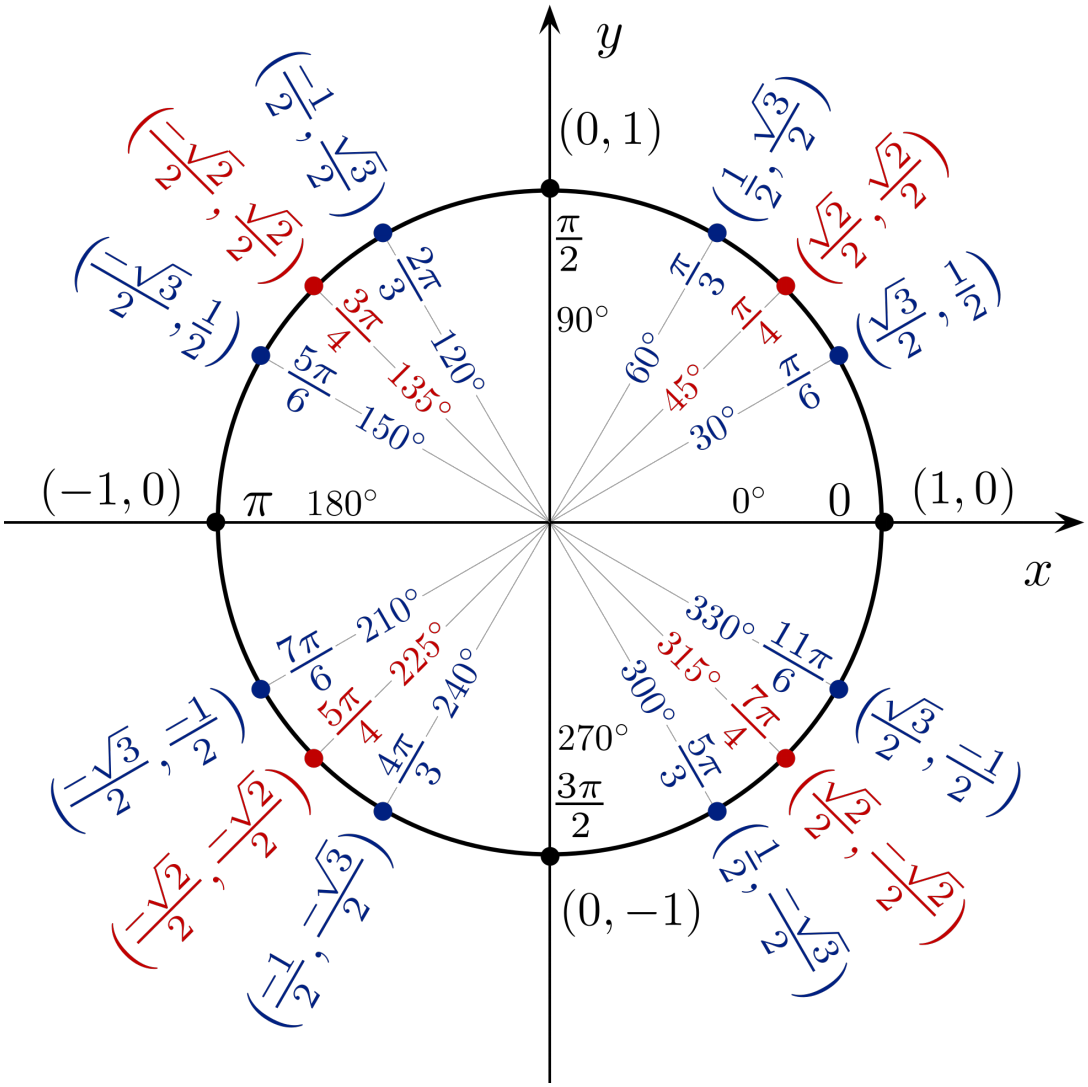
\includegraphics[scale=0.225]{sinus_cosinus}

\sep

\Satz[3.8.2] Eigenschaften von sin und cos
\begin{enumerate}
	\item $\cos z = \cos(-z) \text{ und } \sin(-z) = -\sin(z)$
	\item $\exp(i \cdot z) = \cos(z) + i \cdot \sin(z)$
	\item $\cos(z)^2 + \sin(z)^2 = 1$
	\item $\sin(z+w) = \sin(z) \cdot \cos(w) + \sin(w) \cdot \cos(z)$ \\
	 $\cos(z+w) = \cos(z) \cdot \cos(w) - \sin(w) \cdot \sin(z)$ 
	\item $\sin(z) = \frac{e^{iz}-e^{-iz}}{2i}$, $\cos(z) = \frac{e^{iz}+e^{-iz}}{2}$
\end{enumerate}

\Korollar[3.8.3] \\
\( \sin(2 \cdot z) = 2 \sin(z) \cdot \cos(z) \) \\ 
\(\cos(2 \cdot z) = \cos(z)^2- \sin(z)^2 \)

\sep

\[\sin(t) = t - \frac{t^3}{6} \cos \theta \quad \text{für ein } \theta \in [0,t] \]

\[\sin(x) \leq x \quad \forall  x \geq 0 \]

\[\abs{\sin(x)} \leq \abs{x} \]
\sep

\subsection{Formula for $a x^2 + b x + c = 0$}

\[ x = \frac{-b + \pm \sqrt{b^2 - 4 a c} }{2 a} \]

\sep

\subsection{Konvergente Folgen}
\begin{enumerate}
\item Weierstrass (monoton + beschränkt)
\item Vergleichssatz
\end{enumerate}

\sep

\subsection{Konvergente Reihen}

\begin{enumerate}
\item Weierstrass (monoton + beschränkt)
\item Vergleichssatz
\item Geometrische Folge
\item Alternierende Reihe
\item Riemann Zeta
\item Teleskopieren
\item $\lim \limits_{n \rightarrow \infty} a_n = 0$
\item konvergiert das Integral?
\end{enumerate}

\sep

\subsection{Implications}

\( \text{f differenzierbar} \implies \text{f stetig} \implies \text{f integrierbar} \)

\sep

\subsection{Länge von Kurven}

\[ L = \int_a^b = \sqrt{x'(t)^2 + y'(t)^2} dt  \quad p(t) = (x(t), y(t))\]

\[ L = \int_c^d = \sqrt{1 + f'(x)^2} dx \quad y = f(x), \ x \in [c, d] \]


\end{multicols*}
\end{document}
